% =====================================================================
%  แผนงานกลุ่ม — ตรวจจับ wash trading บน Polymarket (01204465 Assignment #2)
%
%  Build (from Project/plan/):
%    latexmk -xelatex -outdir=build group_plan.tex && cp build/group_plan.pdf .
%
%  Figure sources:
%    figures/theta_sensitivity.png, figures/top_markets.png
%      ← plan/make_figures.py, which reads 04_Evaluation/premise_test/results/*
%    everything else is hand-drawn TikZ in this file
%
%  Every premise-test number in Part 3 comes from those result files. If the
%  pipeline is re-run and they change, re-run make_figures.py and update the
%  prose and tables here to match.
% =====================================================================

\documentclass[11pt,a4paper]{article}

% ---------------------------------------------------------------------
%  FONTS — TLWG dual-script families (Thai + Latin in one file)
% ---------------------------------------------------------------------
\usepackage{fontspec}
\setmainfont{Laksaman}[Ligatures=TeX]
\setsansfont{Garuda}[Ligatures=TeX]
\setmonofont{DejaVu Sans Mono}[Scale=0.84]

\XeTeXlinebreaklocale "th"
\XeTeXlinebreakskip = 0pt plus 0.15em minus 0.02em
\emergencystretch=2.2em

\newcommand{\sansall}{\sffamily}

% ---------------------------------------------------------------------
%  LAYOUT
% ---------------------------------------------------------------------
\usepackage[a4paper,margin=2.3cm,top=2.5cm,bottom=2.5cm,headsep=12pt]{geometry}
\usepackage{amsmath,amssymb}
\usepackage{graphicx}
\graphicspath{{figures/}}
\usepackage{booktabs}
\usepackage{array}
\usepackage{longtable}
\usepackage{multirow}
\usepackage{xcolor}
\usepackage{tikz}
\usetikzlibrary{arrows.meta,positioning,calc,shapes.geometric,shapes.misc,
                fit,backgrounds,decorations.pathmorphing}
\usepackage[most]{tcolorbox}
\usepackage[font=small,labelfont=bf,width=0.95\textwidth]{caption}
\usepackage{fancyhdr}
\usepackage{enumitem}
\usepackage{titlesec}
\usepackage{float}
\usepackage{microtype}
\usepackage[colorlinks=true,allcolors=accent,breaklinks=true,
            bookmarksnumbered=true]{hyperref}

\linespread{1.28}
\setlength{\parskip}{0.35em}
\setlength{\parindent}{0pt}

% ---------------------------------------------------------------------
%  COLOUR — one hue per role / pipeline stage (Okabe–Ito, colour-blind safe)
%  Same hex values as plan/make_figures.py.
% ---------------------------------------------------------------------
\definecolor{accent}{HTML}{0072B2}   % blue   — data pipeline, person A
\definecolor{alg}{HTML}{D55E00}      % orange — Algorithm 1, person B
\definecolor{evalc}{HTML}{009E73}    % green  — evaluation
\definecolor{ext}{HTML}{7B5EA7}      % purple — EDA + chip dumping, person C

\definecolor{ink}{HTML}{1A2733}
\definecolor{muted}{HTML}{5B6B7A}
\definecolor{rule}{HTML}{C9D2DB}
\definecolor{wash}{HTML}{F1F6FA}
\definecolor{warnwash}{HTML}{FDF3E7}
\definecolor{goodwash}{HTML}{E9F4F0}
\definecolor{badwash}{HTML}{FBEDED}
\definecolor{bad}{HTML}{B3261E}

% ---------------------------------------------------------------------
%  HEADINGS
% ---------------------------------------------------------------------
\renewcommand{\thepart}{\arabic{part}}
\titleformat{\part}[display]
  {\sansall\huge\bfseries\color{accent}}
  {\normalsize\color{muted}ภาคที่ \thepart}{0.4em}{}
\titlespacing*{\part}{0pt}{0pt}{1.2em}

\titleformat{\section}
  {\sansall\Large\bfseries\color{accent!88!black}}{\thesection}{0.7em}{}
\titleformat{\subsection}
  {\sansall\large\bfseries\color{ink}}{\thesubsection}{0.6em}{}
\titleformat{\subsubsection}
  {\sansall\normalsize\bfseries\color{muted}}{\thesubsubsection}{0.55em}{}
\titlespacing*{\section}{0pt}{1.9em}{0.7em}
\titlespacing*{\subsection}{0pt}{1.3em}{0.45em}
\titlespacing*{\subsubsection}{0pt}{1.0em}{0.35em}

\pagestyle{fancy}
\fancyhf{}
\renewcommand{\headrulewidth}{0.4pt}
\fancyhead[L]{\footnotesize\sansall\color{muted}แผนงานกลุ่ม · Polymarket wash trading}
\fancyhead[R]{\footnotesize\sansall\color{muted}\leftmark}
\fancyfoot[C]{\footnotesize\color{muted}\thepage}
\renewcommand{\sectionmark}[1]{\markboth{#1}{}}

\setlist[itemize]{itemsep=1pt,topsep=3pt,parsep=0pt,leftmargin=1.4em}
\setlist[enumerate]{itemsep=1pt,topsep=3pt,parsep=0pt,leftmargin=1.6em}
\setlist[description]{itemsep=2pt,topsep=3pt,parsep=0pt}

% ---------------------------------------------------------------------
%  CALLOUT BOXES — four fixed meanings
% ---------------------------------------------------------------------
\tcbset{guidebox/.style={
  enhanced, breakable, boxrule=0pt, leftrule=2.5pt, arc=1pt,
  left=8pt, right=8pt, top=6pt, bottom=6pt,
  fonttitle=\sansall\bfseries\small, titlerule=0pt,
  toptitle=1pt, bottomtitle=1pt}}
\newtcolorbox{keybox}[1][]{guidebox, colback=wash, colframe=accent,
  colbacktitle=wash, coltitle=accent!85!black, #1}
\newtcolorbox{warnbox}[1][]{guidebox, colback=warnwash, colframe=alg,
  colbacktitle=warnwash, coltitle=alg!80!black, #1}
\newtcolorbox{goodbox}[1][]{guidebox, colback=goodwash, colframe=evalc,
  colbacktitle=goodwash, coltitle=evalc!65!black, #1}
\newtcolorbox{badbox}[1][]{guidebox, colback=badwash, colframe=bad,
  colbacktitle=badwash, coltitle=bad, #1}

% ---------------------------------------------------------------------
%  SEMANTIC MARKUP
% ---------------------------------------------------------------------
\newcommand{\en}[1]{#1}
\newcommand{\code}[1]{\texttt{#1}}
\newcommand{\stg}[2]{\textcolor{#1}{\textbf{\en{#2}}}}
% roles — same colour as their pipeline stage
\newcommand{\rA}{\stg{accent}{A}}
\newcommand{\rB}{\stg{alg}{B}}
\newcommand{\rC}{\stg{ext}{C}}
% stages
\newcommand{\sPre}{\stg{accent}{pre-processing}}
\newcommand{\sAlg}{\stg{alg}{Algorithm 1}}
\newcommand{\sEval}{\stg{evalc}{evaluation}}
\newcommand{\sExt}{\stg{ext}{chip dumping}}

% ---------------------------------------------------------------------
%  DIAGRAM GRAMMAR
% ---------------------------------------------------------------------
\tikzset{
  blk/.style={draw=rule, line width=0.6pt, rounded corners=2.5pt,
              fill=wash, minimum height=9mm, inner xsep=6pt, inner ysep=4pt,
              align=flush center, font=\sansall\footnotesize},
  stage/.style={blk, fill=accent!8, draw=accent!45},
  ar/.style={-{Stealth[length=2.2mm,width=1.8mm]}, line width=0.7pt,
             draw=muted},
  lbl/.style={font=\sansall\scriptsize, text=muted, align=flush center},
  tag/.style={font=\sansall\scriptsize\bfseries, align=flush center},
  wal/.style={circle, draw=#1!70, fill=#1!12, line width=0.7pt,
              minimum size=8mm, inner sep=0pt, font=\sansall\scriptsize},
}

\newcolumntype{L}[1]{>{\raggedright\arraybackslash}p{#1}}
\captionsetup{skip=6pt}

\renewcommand{\figurename}{รูปที่}
\renewcommand{\tablename}{ตารางที่}
\renewcommand{\refname}{เอกสารอ้างอิง}

% table header cell
\newcommand{\thd}[1]{\sansall\bfseries #1}

\begin{document}

% =====================================================================
%  TITLE PAGE
% =====================================================================
\begin{titlepage}
\thispagestyle{empty}
\begin{tikzpicture}[remember picture, overlay]
  \fill[accent!8] (current page.north west) rectangle
       ([yshift=-9.5cm]current page.north east);
  \fill[accent] ([yshift=-9.5cm]current page.north west) rectangle
       ([yshift=-9.62cm]current page.north east);
\end{tikzpicture}

\vspace*{1.2cm}
{\sansall\color{muted}\small เอกสารเสนอเพื่อนร่วมกลุ่ม · 01204465 Data Mining · Group Assignment \#2}

\vspace{0.9cm}
{\sansall\bfseries\fontsize{25}{34}\selectfont\color{accent!90!black}
ตรวจจับการซื้อขายสมรู้ร่วมคิด\\(wash trading) บน Polymarket\par}

\vspace{0.5cm}
{\sansall\fontsize{13.5}{20}\selectfont\color{ink}
แผนงาน · เนื้อหา · ผลเบื้องต้น\\
ตั้งแต่ข้อมูล on-chain ดิบจนถึงวันส่งงาน 19 ต.ค.\par}

\vspace{2.6cm}

\begin{minipage}{0.66\textwidth}
เอกสารนี้สรุปว่าเราจะทำอะไร ใช้ข้อมูลและวิธีอะไร แบ่งงานกันอย่างไร
และต้องเสร็จอะไรภายในวันไหน เพื่อให้ทั้งกลุ่มตกลงแผนร่วมกันก่อนส่งหัวข้อ
วันจันทร์ที่ 5 ต.ค.

\vspace{0.6em}
ตัวเลขในภาคที่ 3 เป็น\textbf{ผลรันจริง}ของ premise test (30 ก.ย.) ไม่ใช่ค่าสมมติ
ส่วนภาคที่ 4 คือไทม์ไลน์ การแบ่งงาน ความเสี่ยง และสิ่งที่ต้องตัดสินใจในที่ประชุม
\end{minipage}

\vfill
\begin{tikzpicture}
  \draw[rule, line width=0.6pt] (0,0) -- (\textwidth,0);
\end{tikzpicture}
\vspace{0.3em}

{\sansall\footnotesize\color{muted}
โครงงาน: \code{data mining/Project/} (branch \code{project/polymarket-wash}) \\
ข้อมูล: Hugging Face \code{moose-code/polymarket-onchain-v1} · สถานะ: premise test ผ่านแล้ว รอส่งหัวข้อ \\
อัปเดตล่าสุด: 30 กันยายน 2569}
\end{titlepage}

% =====================================================================
%  TOC
% =====================================================================
\setcounter{tocdepth}{1}
\microtypesetup{protrusion=false}
{\hypersetup{allcolors=ink}
\renewcommand{\contentsname}{สารบัญ}
\tableofcontents}
\microtypesetup{protrusion=true}
\clearpage

% =====================================================================
%  PART 1 — THE PROBLEM
% =====================================================================
\part{โจทย์: เราจะทำอะไร และทำไม}

\textbf{คำถามของภาคนี้: งานชิ้นนี้คืออะไร และทำไมมันตอบใบงานได้ครบทุกข้อ?}

\section{สรุปทั้งโครงงานในหน้าเดียว}

\begin{keybox}[title={ประโยคเดียวที่ต้องจำ: ``ราวหนึ่งในสี่ของ volume บน Polymarket อาจเป็นของปลอม'' --- เราจะวัดเองว่าจริงไหม}]
เราจะเขียนวิธีตรวจจับ wash trading แบบเครือข่าย (Algorithm 1 ของ Sirolly et al., 2025)
ขึ้นใหม่เองจาก pseudo-code รันบนข้อมูล on-chain สาธารณะ
แล้ว\textbf{พิสูจน์ว่าผลเชื่อถือได้}ทั้งที่ไม่มี ground truth
ด้วยการประเมิน 3 แบบ จากนั้นขยายไปที่มุมการโอนมูลค่าแฝง (chip dumping)
ด้วยเทคนิค clustering และกราฟ
\end{keybox}

\begin{table}[H]
\centering\small
\begin{tabular}{L{3.2cm}L{11.4cm}}
\toprule
\thd{เรื่อง} & \thd{สรุป} \\
\midrule
หัวข้อที่จะส่ง & ตรวจจับการซื้อขายสมรู้ร่วมคิด (wash trading) และการโอนมูลค่าแฝง (chip dumping) บน Polymarket \\
\addlinespace
ข้อมูล & event on-chain ของ Polymarket บน Polygon (Hugging Face, CC-BY-4.0) --- ทุก fill ของ order book, หลายล้านแถวต่อเดือน \\
\addlinespace
ประเภท complex data & กราฟ (กระเป๋า $\times$ กระเป๋า) · อนุกรมเวลา · ข้อมูลไม่สมดุล · ข้อมูลขนาดใหญ่ \\
\addlinespace
เทคนิคหลัก (นอกห้อง) & iterative network score (Algorithm 1) · Louvain community detection · Isolation Forest \\
\addlinespace
เทคนิคในห้อง & k-means / DBSCAN จัดกลุ่มกระเป๋า · evaluation (precision, recall) \\
\addlinespace
ผลเบื้องต้น & สัปดาห์พีค (ธ.ค. 2024) ถูกติดธง \textbf{61.8\%} · สัปดาห์เงียบ (มิ.ย. 2025) \textbf{0.35\%} --- ตรงกับเปเปอร์ ($\approx$60\% และ $<$5\%) \\
\addlinespace
เดดไลน์ & ส่งหัวข้อ + รายชื่อ \textbf{จ. 5 ต.ค.} · ส่งวิดีโอ + สไลด์ + รายงาน \textbf{จ. 19 ต.ค.} \\
\bottomrule
\end{tabular}
\caption{ภาพรวมของโครงงาน --- ทุกบรรทัดในตารางนี้มีหัวข้อขยายในภาคต่อ ๆ ไป}
\end{table}

\section{Polymarket กับ wash trading คืออะไร}

\subsection{ตลาดทำนายผลซื้อขายอะไรกันแน่}

Polymarket เป็นตลาดทำนายผล (prediction market) ทุกคำถาม เช่น
``Will the Falcons win Super Bowl 2025?'' มี\textbf{หุ้นสองฝั่ง} คือ Yes กับ No
เมื่อคำถามได้คำตอบ หุ้นฝั่งที่ถูกจะมีค่า \$1 ส่วนฝั่งที่ผิดจะมีค่า \$0
ราคาหุ้นก่อนตลาดปิดจึงสะท้อนความน่าจะเป็นที่ตลาดเชื่อ

การซื้อขายทำผ่าน order book (CLOB) และทุกการจับคู่คำสั่งถูกบันทึกลงบล็อกเชน Polygon
แปลว่า\textbf{ใครเทรดกับใคร เท่าไร เมื่อไร เห็นได้หมด} --- นี่คือสิ่งที่ทำให้โจทย์นี้ทำได้
เพราะข้อมูลตลาดหุ้นทั่วไปไม่เปิดเผยตัวตนของคู่เทรด

\subsection{wash trading หน้าตาเป็นอย่างไรในข้อมูล}

wash trading คือการซื้อขายกับตัวเองหรือกับพวกเดียวกันเพื่อ\textbf{สร้าง volume ปลอม}
โดยที่สุดท้ายไม่มีใครถือความเสี่ยงจริง เหตุจูงใจที่มักถูกพูดถึงคือการปั่น volume
ให้ตลาดดูคึกคัก หรือหวังรางวัลที่แจกตามปริมาณการเทรด
Polymarket บล็อกการเทรดกับกระเป๋าตัวเองแล้ว (self-trade ในข้อมูลของเรา $=0$)
จึงต้องใช้\textbf{หลายกระเป๋าเทรดวนกันเอง}แทน

\begin{figure}[H]
\centering
\begin{tikzpicture}[x=1cm,y=1cm]
  % --- วง wash: สามกระเป๋าเทรดวนกัน ---
  \node[wal=alg] (a) at (0,0) {W1};
  \node[wal=alg] (b) at (2.4,0) {W2};
  \node[wal=alg] (c) at (1.2,1.8) {W3};
  \draw[ar, draw=alg, bend left=18] (a) to node[lbl, below=1pt]{ซื้อ 100} (b);
  \draw[ar, draw=alg, bend left=18] (b) to node[lbl, right=1pt]{ขาย 100} (c);
  \draw[ar, draw=alg, bend left=18] (c) to node[lbl, left=1pt]{ขาย 100} (a);
  \node[tag, text=alg] at (1.2,-1.05) {วง wash};
  \node[lbl, text width=4.4cm] at (1.2,-1.6)
       {เทรดกันเองเกือบทั้งหมด\\position ของทุกคนกลับมาเป็น 0};

  % --- ผู้เล่นจริง ---
  \node[wal=accent] (u1) at (7.0,1.6) {U1};
  \node[wal=accent] (u2) at (9.2,1.6) {U2};
  \node[wal=accent] (u3) at (7.0,-0.2) {U3};
  \node[wal=accent] (u4) at (9.2,-0.2) {U4};
  \draw[ar, draw=accent] (u1) -- (u2);
  \draw[ar, draw=accent] (u3) -- (u2);
  \draw[ar, draw=accent] (u4) -- (u1);
  \draw[ar, draw=accent] (u3) -- (u4);
  \node[tag, text=accent] at (8.1,-1.05) {ผู้เล่นจริง};
  \node[lbl, text width=4.4cm] at (8.1,-1.6)
       {เทรดกับคนหลากหลาย\\ถือ position จนตลาดปิด};

  % --- กล่องอธิบายในรูป ---
  \node[blk, fill=alg!6, draw=alg!40, text width=11.2cm] at (4.6,-3.1)
       {สัญญาณที่ใช้จับมีสองชั้น: (1) \textbf{ปิด position จนเกือบเป็นศูนย์}
        ในตลาดที่เทรด (2) \textbf{คู่เทรดส่วนใหญ่ก็มีพฤติกรรมแบบเดียวกัน}\\[3pt]
        \scriptsize\color{muted}ชั้นแรกอย่างเดียวจับนักเก็งกำไรระยะสั้นผิดตัวได้ ---
        ชั้นที่สอง (เครือข่าย) คือสิ่งที่ Algorithm 1 เพิ่มเข้ามา};
\end{tikzpicture}
\caption{wash trading ต่างจากการเทรดจริงที่ \emph{รูปแบบเครือข่าย} ไม่ใช่ที่เทรดใดเทรดหนึ่ง
--- จึงต้องใช้วิธีระดับกราฟ ไม่ใช่กฎรายแถว}
\label{fig:washnet}
\end{figure}

\subsection{chip dumping --- มุมที่เราขยายเพิ่ม}

chip dumping คือการ\textbf{ตั้งใจเทรดขาดทุนให้กระเป๋าอีกใบ} เพื่อโอนมูลค่าแบบแนบเนียน
(คำนี้มาจากโป๊กเกอร์ออนไลน์) ในข้อมูลจะเห็นเป็นเงินที่ไหลจากกระเป๋า X ไปกระเป๋า Y
อย่างสม่ำเสมอผ่านการเทรดที่ราคาเสียเปรียบ ส่วนนี้\textbf{ไม่มีงานให้เทียบ}
จึงวางเป็นส่วนขยาย (ของคน \rC) ไม่ใช่แกนหลัก

\begin{warnbox}[title={ทำไมชื่อหัวข้อไม่ใช้คำว่า ``ฟอกเงิน'' ตรง ๆ}]
ถ้าตั้งชื่อว่า ``ตรวจจับการฟอกเงิน'' อาจารย์จะถามหา ground truth ว่ากระเป๋าไหนฟอกเงินจริง
ซึ่งเราไม่มีและหาไม่ได้ สิ่งที่วัดได้และมีเปเปอร์ให้เทียบคือ \textbf{wash trading}
ส่วน chip dumping ใช้คำว่า ``การโอนมูลค่าแฝง'' และเล่าในฐานะการสำรวจ
--- ใครพูดในวิดีโอหรือตอบ Q\&A ให้ใช้คำชุดนี้ให้ตรงกัน
\end{warnbox}

\section{งานนี้ตอบ rubric ข้อไหน ด้วยอะไร}

ใบงานให้คะแนน 6 ข้อ และ template สไลด์ของคณะมี 8 ส่วน
ตารางนี้คือ\textbf{สัญญาของกลุ่ม}: ทุกส่วนมีเนื้อหาและมีเจ้าของแล้ว

\begin{table}[H]
\centering\small
\begin{tabular}{L{3.3cm}L{2.4cm}L{7.4cm}c}
\toprule
\thd{ส่วนในสไลด์} & \thd{rubric (น้ำหนัก)} & \thd{เนื้อหาของเรา} & \thd{เจ้าของ} \\
\midrule
Complex Data? Applications? & Data Complexity (10\%) &
  กราฟกระเป๋า × กระเป๋า · อนุกรมเวลา · ไม่สมดุล · ล้านแถวต่อวัน ·
  ตรงกับตัวอย่าง ``stock market feed'' ในใบงาน & \rC \\
\addlinespace
Complex Data Exploration & Exploration (10\%) &
  volume รายสัปดาห์ · การกระจาย degree · หมวดตลาด · ขนาดเทรด & \rC \\
\addlinespace
Complex Data Pre-Processing & \textbf{Pre-processing (20\%)} &
  ตัดแถวสรุปของ taker · แปลงหน่วย · map token\ensuremath{\to}ตลาด · ไล่ position ·
  หา closure · ขอบหน้าต่างเวลา & \rA \\
\addlinespace
Analytic technique (นอกห้อง) & \textbf{Analytics Technique (20\%)} &
  Algorithm 1 · Louvain · Isolation Forest · (ในห้อง: k-means/DBSCAN) & \rB{} + \rC \\
\addlinespace
Demo with tool/coding & Completeness (20\%) &
  notebook รันจบตัวเดียว ตั้งแต่ข้อมูลดิบถึงกราฟธง & ทุกคน \\
\addlinespace
Evaluation & \textbf{Completeness (20\%)} &
  เทียบ Fig.~7 ของเปเปอร์ · synthetic injection · precision@k & \rB \\
\addlinespace
Possible applications & Presentation (10\%) &
  ระบบเฝ้าระวังของตลาด · หน่วยงานกำกับ · ``volume จริง'' สำหรับนักลงทุน & \rC \\
\addlinespace
วิดีโอ + Q\&A & Presentation + Question (10\%) &
  เล่าเรื่อง ``หนึ่งในสี่ของ volume อาจเป็นของปลอม'' & ทุกคน \\
\bottomrule
\end{tabular}
\caption{rubric \ensuremath{\to} เนื้อหา \ensuremath{\to} เจ้าของ --- ข้อที่น้ำหนักสูงสุดสามข้อ (20\% ต่อข้อ)
ตกอยู่ที่ pre-processing, เทคนิค และ evaluation ซึ่งเป็นแกนของงานนี้พอดี}
\end{table}

``นอกห้อง'' ตัดสินจากเนื้อหาที่สอนแล้วในวิชา ได้แก่ association rules, decision tree,
k-NN, k-means, DBSCAN, PCA, regression และ evaluation ---
Algorithm 1, Louvain และ Isolation Forest จึงนับเป็นเทคนิคนอกห้องทั้งหมด

\section{สิ่งที่ต้องส่ง}

\begin{table}[H]
\centering\small
\begin{tabular}{L{3.4cm}L{7.2cm}L{3.8cm}}
\toprule
\thd{ชิ้นงาน} & \thd{ข้อกำหนด (สมมติตามงานกลุ่ม \#1)} & \thd{ส่งวันที่} \\
\midrule
หัวข้อ + รายชื่อ 3 คน & หน้าเดียว: ชื่อหัวข้อ ข้อมูล ประเภท complex data เทคนิคหลัก ·
  ส่งทาง Google Classroom (code \code{aulxievt}) & \textbf{จ. 5 ต.ค.} \\
\addlinespace
สไลด์ (PPT) & template ของคณะ 8 ส่วน รวมราว 15--20 สไลด์ & \textbf{จ. 19 ต.ค.} \\
\addlinespace
รายงาน (PDF) & 10--15 หน้า & \textbf{จ. 19 ต.ค.} \\
\addlinespace
วิดีโอ & 8--15 นาที ทุกคนพูดส่วนของตัวเอง มีช่วง demo & \textbf{จ. 19 ต.ค.} \\
\addlinespace
AI Usage Log & อย่างน้อย 5 prompts บันทึก\textbf{ระหว่างทำ} ไม่ใช่ย้อนเขียน & \textbf{จ. 19 ต.ค.} \\
\addlinespace
โฟลเดอร์ Drive & \code{GroupXX\_ProjectName/} โครงเดียวกับโฟลเดอร์ \code{01}--\code{08} ในโปรเจกต์ & \textbf{จ. 19 ต.ค.} \\
\bottomrule
\end{tabular}
\caption{ชิ้นงานที่ต้องส่ง --- ใบงาน \#2 ไม่ได้ระบุรูปแบบ จึงใช้ของงาน \#1 ไปก่อน}
\end{table}

\begin{warnbox}[title={ต้องถาม TA ให้ได้คำตอบก่อน 5 ต.ค.}]
ใบงาน \#2 ไม่ได้บอกความยาวรายงาน ความยาววิดีโอ ภาษา เรื่อง AI log
และมีนำเสนอสดในสัปดาห์ที่ 14 หรือไม่ ทุกตัวเลขในตารางข้างบนจึงเป็น\textbf{ข้อสมมติ}
ถ้า TA ตอบต่างออกไป ให้แก้ตารางนี้กับ \code{PROGRESS.md} ทันที
\end{warnbox}

% =====================================================================
%  PART 2 — THE CONTENT, FOLLOWING THE DATA
% =====================================================================
\clearpage
\part{เนื้อหา: จากข้อมูลบนบล็อกเชนถึงธง wash}

\textbf{คำถามของภาคนี้: ข้อมูลเดินผ่านขั้นตอนอะไรบ้าง ก่อนจะกลายเป็นคำตอบว่า
``เทรดนี้เป็น wash''?}

ภาคนี้เรียงตามทางเดินของข้อมูลจริง และแต่ละขั้นใช้สีของคนที่รับผิดชอบ
ใครอยู่ขั้นไหนจะเห็นทันทีว่ารับข้อมูลจากใครและส่งต่อให้ใคร

\begin{figure}[H]
\centering
\begin{tikzpicture}[node distance=5mm]
  \node[blk, fill=muted!8, draw=muted!40, text width=2.3cm] (raw)
       {\textbf{ข้อมูลดิบ}\\\scriptsize fill บน Polygon};
  \node[blk, fill=accent!10, draw=accent!45, text width=2.5cm, right=of raw] (pre)
       {\textbf{\sPre}\\\scriptsize คน \rA};
  \node[blk, fill=alg!10, draw=alg!45, text width=2.5cm, right=of pre] (alg)
       {\textbf{\sAlg}\\\scriptsize คน \rB};
  \node[blk, fill=evalc!10, draw=evalc!45, text width=2.5cm, right=of alg] (ev)
       {\textbf{\sEval}\\\scriptsize \rB{} + \rC};
  \node[blk, fill=ext!10, draw=ext!45, text width=2.5cm, below=11mm of pre] (eda)
       {\textbf{EDA}\\\scriptsize คน \rC{} · ทำก่อน};
  \node[blk, fill=ext!10, draw=ext!45, text width=2.5cm, below=11mm of ev] (ext)
       {\textbf{\sExt}\\\scriptsize คน \rC{} · ส่วนขยาย};

  \draw[ar] (raw) -- (pre);
  \draw[ar] (pre) -- (alg);
  \draw[ar] (alg) -- (ev);
  \draw[ar] (raw.south) |- (eda.west);
  \draw[ar, dashed] (eda.north) -- node[lbl, right=1pt, pos=0.4] {ข้อสังเกต} (pre.south);
  \draw[ar] (alg.south) |- (ext.west);

  \node[lbl, above=1.5mm of raw, text width=2.4cm] {§\ref{sec:data}};
  \node[lbl, above=1.5mm of pre, text width=2.4cm] {§\ref{sec:pre}--\ref{sec:closure}};
  \node[lbl, above=1.5mm of alg, text width=2.4cm] {§\ref{sec:alg}};
  \node[lbl, above=1.5mm of ev, text width=2.4cm] {§\ref{sec:eval}};
  \node[lbl, below=1.5mm of eda, text width=2.6cm] {§\ref{sec:eda}};
  \node[lbl, below=1.5mm of ext, text width=2.6cm] {§\ref{sec:ext}};
\end{tikzpicture}
\caption{ทางเดินของข้อมูลและเจ้าของแต่ละขั้น --- EDA อยู่ต้นทางเพราะสิ่งที่เจอต้องย้อนกลับไปปรับ
pre-processing ได้ทัน ส่วน chip dumping อยู่ปลายทางเพราะต้องใช้คะแนนจาก Algorithm 1
ตารางเทรดที่สะอาดของคน \rA{} เป็นจุดที่ทุกคนต้องพึ่ง จึงต้องเสร็จก่อนและต้องถูกที่สุด}
\end{figure}

\section{ข้อมูล: ใช้อะไร ช่วงไหน และทำไม}
\label{sec:data}

\subsection{แหล่งข้อมูล}

ชุดข้อมูล \code{moose-code/polymarket-onchain-v1} บน Hugging Face (CC-BY-4.0)
เป็น event บน Polygon ของ Polymarket ตั้งแต่ ก.ย. 2020 ถึง เม.ย. 2026 เราใช้สามตาราง

\begin{table}[H]
\centering\small
\begin{tabular}{L{4.6cm}L{6.4cm}L{3.2cm}}
\toprule
\thd{ตาราง} & \thd{ใช้ทำอะไร} & \thd{ขนาด} \\
\midrule
\code{order\_filled/year=/month=} & ทุก fill ของ order book --- นี่คือ ``เทรด'' & 0.6--1.4 GB/เดือน ในช่วงที่เลือก \\
\addlinespace
\code{condition.parquet} & token id \ensuremath{\to} (ตลาด, ฝั่ง Yes/No) ผ่าน \code{positionIds} & 126 MB \\
\addlinespace
\code{market\_data.parquet} & ชื่อคำถาม slug หมวด (ใช้ใน EDA) & 137 MB \\
\bottomrule
\end{tabular}
\caption{ตารางที่ใช้ --- ไม่ใช้ \code{user\_position} (12 GB) เป็นข้อมูลหลัก
เพราะต้องคำนวณ position เองอยู่แล้ว แต่ใช้สุ่มเทียบเป็น sanity check ได้}
\end{table}

\subsection{ทำไมเลือกสองช่วงนี้ --- ความต่างคือหลักฐานในตัว}

เปเปอร์รายงานว่า wash trading พีคราว 60\% ของ volume รายสัปดาห์ใน ธ.ค. 2024
และลดเหลือต่ำกว่า 5\% ตั้งแต่ พ.ค. 2025 เราจึงเลือก\textbf{ช่วงพีคคู่กับช่วงเงียบ}
ถ้าวิธีของเราถูก มันต้องติดธงช่วงพีคมากกว่าช่วงเงียบอย่างชัดเจน
โดยไม่ต้องมีป้ายคำตอบรายเทรด

\begin{table}[H]
\centering\small
\begin{tabular}{L{2.8cm}L{3.2cm}L{5.8cm}r}
\toprule
\thd{บทบาท} & \thd{ช่วง} & \thd{เหตุผล} & \thd{ขนาด} \\
\midrule
\textbf{ช่วงพีค} & พ.ย.--ธ.ค. 2024 & เปเปอร์วัด wash ได้ $\approx$60\% --- มีของให้จับเยอะ & 2.4 GB \\
\textbf{ช่วงเงียบ} & พ.ค.--มิ.ย. 2025 & เปเปอร์วัดได้ $<$5\% --- เป็นกลุ่มควบคุม & 1.2 GB \\
ช่วงเสริม (ถ้าทัน) & ต.ค. 2025 & กลับมา $\approx$20\% เป็นจุดวัดที่สาม & 2.0 GB \\
\textcolor{bad}{ไม่ใช้} & ปี 2026 ทั้งหมด & 9--21 GB ต่อเดือน และไม่มีตัวเลขเปเปอร์ให้เทียบ & --- \\
\bottomrule
\end{tabular}
\caption{ช่วงเวลาที่ใช้ รวมช่วงหลักราว 3.6 GB --- เครื่องที่มี RAM 30 GB กับ DuckDB รับได้สบาย}
\end{table}

\subsection{ทำไมข้อมูลนี้นับเป็น complex data}

\begin{itemize}
\item \textbf{กราฟ} --- กระเป๋าเป็นโหนด การเทรดเป็นเส้นเชื่อม
      สัปดาห์พีคมี 334,362 กระเป๋า
\item \textbf{อนุกรมเวลา} --- position ของแต่ละกระเป๋าต้องไล่ตามลำดับบล็อก
      และผลวัดเป็นซีรีส์รายสัปดาห์
\item \textbf{ไม่สมดุล} --- ในช่วงเงียบ wash มีไม่ถึง 1\% ของ volume
\item \textbf{ขนาดใหญ่} --- ราว 17 ล้านแถวดิบสำหรับหน้าต่างเดียว
\end{itemize}

\section{EDA: สำรวจข้อมูลก่อนลงมือ}
\label{sec:eda}

\textbf{เจ้าของ: คน \rC} · rubric Exploration (10\%) · \textbf{เริ่มได้ทันที}
บนตารางเทรดสองสัปดาห์ที่มีอยู่แล้วใน \code{data/interim/} ไม่ต้องรอใคร

\subsection{ทำไม EDA ต้องมาก่อน ไม่ใช่ท้าย}

\begin{itemize}
\item \textbf{ลำดับของ data mining} --- ต้องรู้จักข้อมูลก่อน จึงรู้ว่าต้อง clean อะไร
      และวิธีไหนเหมาะ template สไลด์ของคณะก็เรียง Exploration ไว้ก่อน Pre-processing
\item \textbf{สิ่งที่เจอต้องย้อนกลับไปแก้ต้นทางได้} --- เช่น degree ที่ผิดปกติ
      หรือตลาดที่ไม่มีชื่อ อาจกลายเป็นงานของ \rA{} หรือจุดที่ \rB{} ต้องตรวจ
      ถ้าทำท้ายสุดจะแก้ไม่ทัน
\item \textbf{ไม่มีอะไรขวาง} --- ข้อมูลสองสัปดาห์ที่ผ่าน premise test แล้วพร้อมใช้ตั้งแต่วันนี้
\end{itemize}

\begin{table}[H]
\centering\small
\begin{tabular}{L{3.6cm}L{5.8cm}L{4.8cm}}
\toprule
\thd{สิ่งที่ดู} & \thd{ตอบคำถามอะไร} & \thd{ส่งต่อให้ใคร / ใช้ที่ไหน} \\
\midrule
volume รายวัน/รายสัปดาห์ & ช่วงพีคกับช่วงเงียบต่างกันแค่ไหนก่อนรันอัลกอริทึม & สไลด์ Exploration \\
\addlinespace
การกระจาย degree ของกระเป๋า & กราฟหางยาวไหม มีกระเป๋าที่เทรดกับคู่เดิมซ้ำ ๆ ไหม & \rB{} --- เข้าใจโครงสร้างของ $B$ \\
\addlinespace
หมวดตลาด (Sports / Election / Crypto) & volume กระจุกอยู่หมวดไหน ตลาดไม่มีชื่อ 39\% กระทบแค่ไหน & \rA{} --- ตัดสินใจเรื่องตลาดไร้ชื่อ \\
\addlinespace
การกระจายขนาดเทรดและราคา & มีเทรดขนาดเท่ากันซ้ำ ๆ หรือราคาสุดขั้ว (ใกล้ 0 หรือ 1) ไหม & \rB{} --- ตลาดโอกาสน้อยที่ wash ชอบ \\
\addlinespace
อายุตลาดเทียบกับหน้าต่างเวลา & ตลาดกี่ \% เปิดก่อน lead-in & \rA{} --- ขนาดของปัญหาขอบหน้าต่าง \\
\bottomrule
\end{tabular}
\caption{EDA รอบแรก --- ทุกกราฟวางสองหน้าต่างเวลาข้างกัน
และทุกข้อมีคนรับข้อสังเกตต่อ ไม่ใช่ทำไว้ใส่สไลด์อย่างเดียว}
\end{table}

\begin{keybox}[title={EDA มีสองรอบ}]
\textbf{รอบแรก (ถึง 4 ต.ค.)} --- บนข้อมูลสองสัปดาห์ที่มีอยู่
ส่งรายการข้อสังเกตให้ \rA{} และ \rB{}\\[3pt]
\textbf{รอบสอง (ถึง 10 ต.ค.)} --- รันกราฟชุดเดิมบนช่วงเต็มที่ \rA{} ส่งมา
และเพิ่มกราฟเทียบกระเป๋าที่ถูกติดธงกับไม่ถูกติดธง (ส่วนนี้ส่วนเดียวที่ต้องรอผลของ \rB)
\end{keybox}

\section{Pre-processing: จากแถวดิบเป็นตารางเทรดที่สะอาด}
\label{sec:pre}

\textbf{เจ้าของ: คน \rA} · rubric ข้อที่หนักที่สุดข้อหนึ่ง (20\%) และเป็นส่วนที่มีเรื่องเล่าเยอะที่สุด

\subsection{ข้อมูลดิบมีกับดักอะไรบ้าง}

\begin{table}[H]
\centering\small
\begin{tabular}{L{4.4cm}L{5.0cm}L{5.0cm}}
\toprule
\thd{ปัญหาในข้อมูลดิบ} & \thd{ถ้าไม่แก้จะเกิดอะไร} & \thd{ที่เราทำ} \\
\midrule
แถวที่ \code{taker} เป็นสัญญา exchange เป็นแถว\textbf{สรุป}ของคำสั่ง taker &
  นับ volume ซ้ำ และคู่เทรดเป็น ``สัญญา'' แทนคนจริง &
  ตัดทิ้ง --- คู่จริงอยู่ในแถว maker ของ tx เดียวกันแล้ว \\
\addlinespace
จำนวนเก็บเป็นข้อความ หน่วย 6 ตำแหน่งทศนิยม &
  คำนวณไม่ได้ หรือค่าเพี้ยน $10^6$ เท่า &
  cast แล้วหาร $10^6$ \\
\addlinespace
address มีทั้งตัวเล็กตัวใหญ่ &
  กระเป๋าเดียวกันถูกนับเป็นสองใบ &
  แปลงเป็นตัวเล็กทั้งหมด \\
\addlinespace
token id ไม่บอกว่าเป็นตลาดไหน ฝั่งไหน &
  รวม position ข้ามตลาดไม่ได้ &
  map ผ่าน \code{condition.positionIds} (index 0 = Yes, 1 = No) \\
\addlinespace
การจับคู่มีสามแบบ: ซื้อ/ขาย, mint (ซื้อ Yes + ซื้อ No), merge &
  ต้องเขียนตรรกะแยกสามแบบเพื่อหา position ของ taker &
  ใช้ข้อเท็จจริงว่า $\Delta P_{\text{taker}} = -\Delta P_{\text{maker}}$ ทุกแบบ (ดูด้านล่าง) \\
\addlinespace
position ที่เปิดก่อนหน้าต่างเวลา &
  กระเป๋าที่ปิด position ดูเหมือนไม่เคยปิด &
  ดึงข้อมูลเผื่อก่อนหน้า 1 เดือน (lead-in) \\
\bottomrule
\end{tabular}
\caption{กับดักของข้อมูลดิบและวิธีแก้ --- ตารางนี้คือโครงของสไลด์ Pre-processing ได้ทันที}
\end{table}

\subsection{ตัวเลขก่อน--หลังแต่ละขั้น}

\begin{figure}[H]
\centering
\begin{tikzpicture}[x=1cm,y=1cm]
  % ความกว้างของแถบ ∝ จำนวนแถว (17.21 M = 13 cm)
  \def\s{0.7553}
  \fill[muted!25] (0,0) rectangle (17.214*\s,0.7);
  \node[font=\sansall\footnotesize, anchor=west] at (0.15,0.35)
       {fill ดิบ (1 พ.ย. -- 7 ธ.ค. 2024) \quad \textbf{17,213,896}};

  \fill[bad!20] (0,-1.1) rectangle (7.868*\s,-0.4);
  \node[font=\sansall\footnotesize, anchor=west] at (0.15,-0.75)
       {แถวสรุปของ taker ตัดทิ้ง \quad \textbf{7,867,942}};

  \fill[accent!30] (0,-2.2) rectangle (9.346*\s,-1.5);
  \node[font=\sansall\footnotesize, anchor=west] at (0.15,-1.85)
       {เทรดที่เก็บไว้ \quad \textbf{9,345,954}};

  \fill[accent!60] (0,-3.3) rectangle (1.635*\s,-2.6);
  \node[font=\sansall\footnotesize, anchor=west] at (1.4,-2.95)
       {อยู่ในสัปดาห์เป้าหมาย 1--7 ธ.ค. \quad \textbf{1,635,178} เทรด · 692.9 M shares · 2,307 ตลาด};

  \node[blk, fill=evalc!8, draw=evalc!45, text width=12.4cm, anchor=north west] at (0,-3.75)
       {ตรวจความถูกต้องระหว่างทาง: token ที่ map ไม่ได้ \textbf{0} แถว ·
        self-trade \textbf{0} แถว\\[2pt]
        \scriptsize\color{muted}ทั้งสองตัวเป็น 0 เหมือนกันในหน้าต่าง มิ.ย. 2025
        (10.55 M แถวดิบ \ensuremath{\to} 6.19 M เทรด) --- ตัวเลขชุดนี้ไปอยู่ในสไลด์ได้เลย};
\end{tikzpicture}
\caption{แถวดิบเกือบครึ่งเป็นแถวซ้ำที่ต้องตัด ถ้าไม่ตัด volume จะเกือบเป็นสองเท่า
และคู่เทรดครึ่งหนึ่งจะเป็นสัญญา exchange แทนคนจริง (ตัวเลขจาก \code{extract\_stats.json})}
\end{figure}

\subsection{ทำไม position ของ taker ไม่ต้องคำนวณแยก}

เราวัด position เป็น ``จำนวนหุ้น Yes สุทธิ'' ของแต่ละกระเป๋าในแต่ละตลาด
โดยให้การถือ No นับเป็นค่าลบ (เพราะ Yes 1 หุ้น + No 1 หุ้น = \$1 แน่นอน ไม่มีความเสี่ยง)

\begin{equation}
\Delta P_{\text{maker}} =
\underbrace{(\pm 1)}_{\text{ซื้อ }+1,\ \text{ขาย }-1}
\times
\underbrace{(\pm 1)}_{\text{Yes }+1,\ \text{No }-1}
\times
\underbrace{n}_{\text{จำนวนหุ้น}}
\end{equation}

ตัวอย่างแบบ mint: maker ซื้อ Yes 100 หุ้น taker ซื้อ No 100 หุ้น (ทั้งคู่จ่าย USDC)
maker ได้ $\Delta P = +100$ ส่วน taker ถือ No 100 หุ้นซึ่งนับเป็น $-100$
\textbf{ผลรวมเป็นศูนย์เสมอ} เช่นเดียวกับแบบซื้อ/ขายและ merge

\begin{keybox}[title={ข้อสังเกตที่ทำให้ไปป์ไลน์ง่ายลงครึ่งหนึ่ง}]
ในทุกแบบการจับคู่ ฝั่งหนึ่งได้ position $+n$ อีกฝั่งได้ $-n$
เราจึงเก็บแค่ $\Delta P_{\text{maker}}$ ต่อแถว แล้วใช้ $-\Delta P_{\text{maker}}$ เป็นของ taker
ไม่ต้องสร้างคำสั่งฝั่ง taker ขึ้นใหม่เลย และแต่ละเทรดนับ volume $n$ หุ้น
(ไม่ใช่ $2n$) ตามข้อตกลงของเปเปอร์
\end{keybox}

\section{Closure: สัญญาณชั้นแรกของ wash}
\label{sec:closure}

\subsection{closure คืออะไร}

กระเป๋า $i$ ถือว่า ``ปิด position'' (closure) ในตลาด $m$ ถ้า position ของมัน
\textbf{ลดลงจนเหลือไม่เกิน 0.5\% ของจุดสูงสุดก่อนหน้า} ($c = 0.005$)
หรือกลับฝั่งจาก long เป็น short (ซึ่งต้องผ่านศูนย์)
ผู้เล่นจริงส่วนใหญ่ถือจนตลาดปิด ส่วน wash trader ซื้อแล้วขายคืนจนกลับเป็นศูนย์

\begin{figure}[H]
\centering
\begin{tikzpicture}[x=0.95cm,y=0.028cm]
  % แกน
  \draw[ar] (0,0) -- (13.3,0) node[lbl, right] {เวลา};
  \draw[ar] (0,-5) -- (0,125) node[lbl, above] {position $P$};
  \draw[rule] (0,100) -- (13,100);
  \node[lbl, left] at (0,100) {100};
  \node[lbl, left] at (0,0) {0};

  % กระเป๋า wash: ขึ้นไป 100 แล้วลงมาเหลือ 0.4 \ensuremath{\to} closure
  \draw[alg, line width=1.3pt] (0,0) -- (1,60) -- (2,100) -- (3.2,100) -- (4.2,40) -- (5.2,0.4)
        -- (6.2,0.4);
  \fill[alg] (5.2,0.4) circle (2.2pt);
  \node[tag, text=alg, above right] at (4.9,8) {closure};
  \node[lbl, text=alg!80!black, text width=3.2cm] at (3.1,-22)
       {เหลือ 0.4 $\le$ 0.005 × 100\\$\Rightarrow Q_{im} > 0$};

  % ผู้เล่นจริง: ขึ้นไป 80 แล้วลดเหลือ 70 ถือจนจบ
  \draw[accent, line width=1.3pt] (7,0) -- (8,50) -- (9,80) -- (10.5,70) -- (13,70);
  \node[tag, text=accent, above] at (11.5,72) {ไม่มี closure};
  \node[lbl, text=accent!80!black, text width=3.4cm] at (10.2,-22)
       {ลดจาก 80 เหลือ 70\\ยังถือความเสี่ยงอยู่};
\end{tikzpicture}
\caption{closure เป็นการทดสอบ ``มีหรือไม่มี'' เท่านั้น ($Q_{im} > 0$) --- เราไม่ต้องนับว่าปิดกี่ครั้ง
จึงคำนวณได้ด้วย window function ใน SQL บนหลายสิบล้านแถวในไม่กี่วินาที}
\end{figure}

\begin{warnbox}[title={ข้อจำกัดที่ต้องพูดตรง ๆ: position ก่อนหน้าต่างเวลาเราไม่รู้}]
เราดึงข้อมูลเผื่อก่อนหน้า 1 เดือน แต่ถ้ากระเป๋าเปิด position ก่อนนั้น
จุดสูงสุดที่เราเห็นจะต่ำกว่าความจริง ตลาดที่เปิดยาว (เช่นตลาดการเมือง)
จึงอาจถูกนับ closure มากเกินไป เฟส 2 จะลองขยาย lead-in
และสุ่มเทียบกับตาราง \code{user\_position} เพื่อวัดว่าผลกระทบมากแค่ไหน
\end{warnbox}

\section{Algorithm 1: คะแนนเครือข่าย}
\label{sec:alg}

\textbf{เจ้าของ: คน \rB} · Sirolly et al. (2025) §5.1 --- ไม่มีโค้ดเผยแพร่ เราเขียนเองจาก pseudo-code

\subsection{ส่วนที่ 1 --- คะแนนตั้งต้นจาก closure}

\begin{equation}
x^{0}_i \;=\; \sum_{m}
\underbrace{s_{im}}_{\substack{\text{สัดส่วน volume ของ } i\\ \text{ที่เทรดในตลาด } m}}
\cdot
\underbrace{\mathbf{1}\{Q_{im} > 0\}}_{\substack{\text{เคยปิด position}\\ \text{ในตลาด } m \text{ หรือไม่}}}
\end{equation}

$x^0_i$ จึงอยู่ระหว่าง 0 ถึง 1 และแปลว่า ``volume ของกระเป๋านี้กี่เปอร์เซ็นต์
อยู่ในตลาดที่มันปิด position'' ค่าสูงแปลว่าน่าสงสัย แต่ยังแยกนักเก็งกำไรระยะสั้นไม่ออก

\subsection{ส่วนที่ 2 --- ให้คะแนนไหลผ่านคู่เทรด}

\begin{equation}
x \;\leftarrow\; \tfrac{1}{2}\Big(
\underbrace{x^{0}}_{\text{พฤติกรรมตัวเอง}}
\;+\;
\underbrace{B\,x}_{\substack{\text{ค่าเฉลี่ยคะแนนคู่เทรด}\\ \text{ถ่วงตาม volume}}}
\Big)
\qquad
B_{ij} = \frac{\text{volume ที่ } i \text{ เทรดกับ } j}{\text{volume ทั้งหมดของ } i}
\end{equation}

ทำซ้ำจนการเปลี่ยนแปลงสัมพัทธ์ต่ำกว่า $10^{-5}$ (ของเราใช้ 10--11 รอบ เปเปอร์ใช้ 12)
กระเป๋าที่เทรดกับพวกคะแนนสูงเป็นส่วนใหญ่จะถูกดึงขึ้น
ส่วนนักเก็งกำไรที่เทรดกับคนทั่วไปจะถูกดึงลง --- นี่คือชั้นเครือข่ายในรูปที่~\ref{fig:washnet} (รูปที่~\ref{fig:score} แสดงตัวอย่าง)

\begin{figure}[H]
\centering
\begin{tikzpicture}[x=1cm,y=1cm]
  \node[wal=alg] (a) at (0,0) {.95};
  \node[wal=alg] (b) at (1.8,0.9) {.97};
  \node[wal=alg] (c) at (1.8,-0.9) {.93};
  \node[wal=accent] (d) at (4.6,0) {.90};
  \node[wal=accent] (e) at (6.6,0.9) {.20};
  \node[wal=accent] (f) at (6.6,-0.9) {.15};
  \draw[alg, line width=2pt] (a) -- (b) -- (c) -- (a);
  \draw[muted, line width=0.8pt] (c) -- (d);
  \draw[accent, line width=1.6pt] (d) -- (e);
  \draw[accent, line width=1.6pt] (d) -- (f);
  \node[lbl] at (1.2,-1.8) {วง wash: คะแนนสูงค้ำกันเอง};
  \node[lbl, text width=4.2cm] at (5.8,-2.15)
       {นักเก็งกำไร $x^0 = .90$ แต่คู่เทรดคะแนนต่ำ\\\ensuremath{\to} คะแนนสุดท้ายถูกดึงลงใต้ $\theta$};
  \node[blk, fill=alg!6, draw=alg!40, text width=3.4cm, anchor=west] at (8.0,0)
       {ตัวเลขในวง = $x^0$\\[2pt]\scriptsize\color{muted}ความหนาเส้น = volume ระหว่างคู่};
\end{tikzpicture}
\caption{คะแนนตั้งต้นสูงเท่ากันยังไม่พอ --- สิ่งที่ Algorithm 1 ถามคือ
``คุณเทรดกับใครเป็นหลัก'' ซึ่งเป็นคำถามระดับกราฟ}
\label{fig:score}
\end{figure}

\subsection{ติดธงเทรดไหน}

\begin{equation}
\boxed{\text{เทรดระหว่าง } i \text{ กับ } j \text{ เป็น wash} \iff \min(x_i,\, x_j) \ge \theta}
\end{equation}

premise test ใช้ $\theta = 0.9$ คงที่ ทุกตลาดใช้ค่าเดียวกัน

\begin{keybox}[title={ตัวตรวจว่าเขียนถูก: ค่าเฉลี่ยถ่วง volume ของคะแนนต้องไม่เปลี่ยน}]
เพราะ $B$ สร้างจาก volume ที่สมมาตรแล้วหารด้วยผลรวมแถว
ค่าเฉลี่ยของ $x$ ที่ถ่วงด้วย volume ของแต่ละกระเป๋าจะเท่าเดิมทุกรอบ
(เปเปอร์เรียกว่า Proposition 2) ผลของเรา: ธ.ค. 0.7877 \ensuremath{\to} 0.7877 และ มิ.ย. 0.5848 \ensuremath{\to} 0.5848
ถ้าวันหนึ่งตัวเลขสองตัวนี้ไม่เท่ากัน แปลว่าเมทริกซ์ $B$ ถูกสร้างผิด
\end{keybox}

\subsection{Algorithm 2 --- สิ่งที่คน \rB{} ต้องเพิ่มในเฟส 2}

เปเปอร์ไม่ได้ใช้ $\theta$ เดียวกับทุกตลาด แต่เลือก $\theta$ \textbf{รายตลาด}
ในช่วง $\underline{\theta} = 0.8$ ถึง $\overline{\theta} = 0.99$ ด้วยการทดสอบ spillover
(พารามิเตอร์ $Y = 0.1$, $\zeta = 0.001$) ตลาดที่ไม่มี $\theta$ ไหนผ่านการทดสอบจะไม่ถูกติดธงเลย
ส่วนนี้สำคัญเพราะอธิบายความต่างที่เราเจอในตลาด Trump (§\ref{sec:trump})
--- ก่อนเขียนต้องอ่านสเปกจากเปเปอร์ให้ละเอียด ไม่เดา

\section{ส่วนขยาย: chip dumping และการจัดกลุ่มกระเป๋า}
\label{sec:ext}

\textbf{เจ้าของ: คน \rC} · ใช้ตารางเทรดสะอาดจาก \rA{} และคะแนนจาก \rB

\begin{table}[H]
\centering\small
\begin{tabular}{L{3.0cm}L{5.4cm}L{4.4cm}c}
\toprule
\thd{เทคนิค} & \thd{ใช้ทำอะไร} & \thd{ผลที่ได้} & \thd{ในห้อง?} \\
\midrule
กราฟ net value-flow & ขอบ $i \to j$ = มูลค่า (USDC) ที่ $i$ เสียให้ $j$ สุทธิ &
  กราฟมีทิศทาง ถ่วงน้ำหนัก & --- \\
\addlinespace
Louvain & หา community ที่เทรดกันเองหนาแน่น & กลุ่มกระเป๋าที่น่าจะเป็นวงเดียวกัน & นอก \\
\addlinespace
Isolation Forest & หากระเป๋าผิดปกติจากฟีเจอร์รายกระเป๋า
  (จำนวนคู่เทรด, \% closure, กำไร/ขาดทุน, ขนาดเทรด) & คะแนนความผิดปกติ & นอก \\
\addlinespace
k-means / DBSCAN & จัดกลุ่มกระเป๋าตามพฤติกรรม & ``ประเภทผู้เล่น'' สำหรับเล่าเรื่อง & ใน \\
\bottomrule
\end{tabular}
\caption{เทคนิคของส่วนขยาย --- ใช้ทั้งในและนอกห้อง ตรงกับที่ rubric อยากเห็น}
\end{table}

\begin{warnbox}[title={ส่วนขยายต้องไม่กินเวลาของแกนหลัก}]
chip dumping ไม่มีตัวเลขให้เทียบ ผลที่ได้จึงเป็น ``สิ่งที่น่าสนใจ'' ไม่ใช่ ``ข้อสรุป''
ถ้าเวลาไม่พอ Isolation Forest เป็นสิ่งแรกที่ตัดได้ (ดู §\ref{sec:risk})
แต่ EDA (§\ref{sec:eda}) ตัดไม่ได้ เพราะเป็น rubric 10\%
\end{warnbox}

\section{Evaluation: ไม่มี ground truth แล้วรู้ได้อย่างไรว่าถูก}
\label{sec:eval}

\textbf{เจ้าของ: คน \rB{}} · \rC{} ช่วยตรวจมือ · นี่คือคำถามแรกที่อาจารย์จะถาม และเป็น completeness 20\%

\begin{table}[H]
\centering\small
\begin{tabular}{L{3.0cm}L{4.8cm}L{3.4cm}L{3.2cm}}
\toprule
\thd{วิธี} & \thd{ทำอย่างไร} & \thd{พิสูจน์อะไร} & \thd{มองไม่เห็นอะไร} \\
\midrule
\textbf{1. เทียบเปเปอร์} & plot \% ที่ถูกติดธงรายสัปดาห์ของเราทับ Fig.~7 ของเปเปอร์ แล้วอธิบายส่วนต่าง &
  ทำซ้ำได้บนข้อมูลคนละแหล่ง & ถ้าเปเปอร์ผิด เราก็ผิดตาม \\
\addlinespace
\textbf{2. Synthetic injection} & ฝังวง wash ที่รู้คำตอบ (3--5 กระเป๋าเทรดวนกัน) ลงข้อมูลจริง
  แล้ววัด recall ที่ $\theta$ ต่าง ๆ & จับวงที่รู้คำตอบได้จริง ได้ precision/recall curve &
  วง wash ที่ซับซ้อนกว่าวงที่เราฝัง \\
\addlinespace
\textbf{3. Precision@k} & สุ่มตรวจมือ top-$k$ กระเป๋าที่ถูกติดธง ($k = 30$--50)
  ด้วยเกณฑ์ที่\textbf{เขียนไว้ก่อนเริ่มตรวจ} & ธงที่ขึ้นมีเหตุผลเมื่อคนดู &
  recall (สิ่งที่หลุด) \\
\bottomrule
\end{tabular}
\caption{สามวิธีปิดจุดบอดของกันและกัน --- ไม่มีวิธีไหนพอเดี่ยว ๆ
ความชัดเจนของสัปดาห์พีคเทียบสัปดาห์เงียบ (ภาคที่ 3) เป็นหลักฐานชิ้นที่สี่ในตัว}
\end{table}

\begin{badbox}[title={อย่าตั้งเกณฑ์ตรวจมือหลังจากเห็นผลแล้ว}]
ถ้าดูรายชื่อ top-$k$ ก่อนแล้วค่อยคิดว่า ``แบบไหนนับเป็น wash''
เราจะเผลอตั้งเกณฑ์ให้ผลออกมาดี precision@k จะไม่มีความหมาย
ให้คน \rC{} เขียนเกณฑ์ลง \code{04\_Evaluation/} และ commit ก่อนเปิดดูรายชื่อ
\end{badbox}

% =====================================================================
%  PART 3 — RESULTS SO FAR
% =====================================================================
\clearpage
\part{ผลที่ได้แล้ว: premise test}

\textbf{คำถามของภาคนี้: ก่อนผูกกลุ่มไว้กับหัวข้อนี้ เรามีหลักฐานอะไรแล้วว่ามันเวิร์ก?}

\section{กติกาที่ตั้งไว้ก่อนรัน}

ก่อนเขียนโค้ดสักบรรทัด เราตั้งเกณฑ์ไว้ว่าจะไปต่อก็ต่อเมื่อ

\begin{equation}
\boxed{\text{สัปดาห์ 1--7 ธ.ค. 2024 ถูกติดธง} \ge 30\%
\quad\text{และ}\quad
\text{สัปดาห์ 1--7 มิ.ย. 2025} \le 10\%}
\qquad (\theta = 0.9)
\end{equation}

เกณฑ์หลวมกว่าตัวเลขเปเปอร์ ($\approx$60\% และ $<$5\%) เพราะเราใช้หน้าต่างสั้นกว่า
ถ้าไม่ผ่านและแก้บั๊กแล้วยังไม่เห็นความต่าง แผนคือ\textbf{ไม่ส่งหัวข้อนี้}
และเปลี่ยนไปหัวข้อสำรองทันที

\section{ผล: ผ่านตั้งแต่ 30 ก.ย. เร็วกว่ากำหนด 4 วัน}

\begin{table}[H]
\centering\small
\begin{tabular}{L{6.6cm}rr}
\toprule
 & \thd{1--7 ธ.ค. 2024 (พีค)} & \thd{1--7 มิ.ย. 2025 (เงียบ)} \\
\midrule
เทรดที่เก็บไว้ (lead-in + สัปดาห์เป้าหมาย) & 9,345,954 & 6,194,635 \\
แถวสรุป taker ที่ตัดทิ้ง & 7,867,942 & 4,359,293 \\
token ที่ map ไม่ได้ / self-trade & 0 / 0 & 0 / 0 \\
volume ของสัปดาห์เป้าหมาย (หุ้น) & 692.9 M & 389.8 M \\
จำนวนกระเป๋า & 334,362 & 295,526 \\
คู่ (กระเป๋า, ตลาด) ที่มี closure & 52.8\% & 38.1\% \\
จำนวนรอบจนลู่เข้า (เปเปอร์: 12) & 10 & 11 \\
คะแนนเฉลี่ยถ่วง volume $x^0$ \ensuremath{\to} สุดท้าย & 0.7877 \ensuremath{\to} 0.7877 & 0.5848 \ensuremath{\to} 0.5848 \\
\addlinespace
\textbf{ถูกติดธงที่ $\theta = 0.9$} & \textbf{61.8\%} & \textbf{0.35\%} \\
\textcolor{muted}{ตัวเลขเปเปอร์} & \textcolor{muted}{$\approx$60\%} & \textcolor{muted}{$<$5\%} \\
\bottomrule
\end{tabular}
\caption{ผล premise test (จาก \code{alg1\_results.json} และ \code{extract\_stats.json})
--- รันทั้งสองหน้าต่างเสร็จในราว 15 วินาทีบน 32 threads}
\end{table}

\begin{figure}[H]
\centering
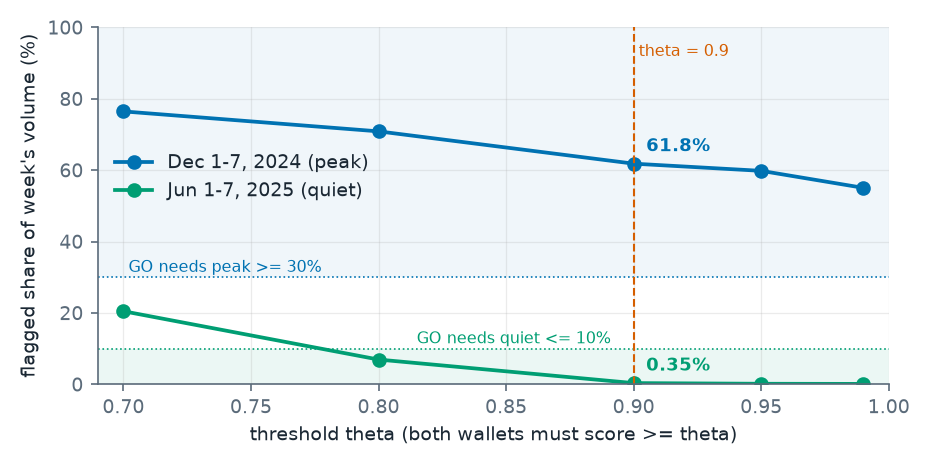
\includegraphics[width=0.92\textwidth]{theta_sensitivity}
\caption{ความต่างระหว่างสองสัปดาห์ไม่ได้ขึ้นกับการเลือก $\theta$ พอดี ---
ที่ทุก $\theta$ ตั้งแต่ 0.8 ขึ้นไป สัปดาห์พีคถูกติดธงเกิน 55\% ขณะที่สัปดาห์เงียบต่ำกว่า 7\%
ส่วนที่ $\theta = 0.7$ สัปดาห์เงียบขึ้นไปถึง 20\% ซึ่งเป็นเหตุผลที่ไม่ใช้ $\theta$ ต่ำ}
\end{figure}

\begin{goodbox}[title={ผ่านเกณฑ์ชัดเจน และใกล้ตัวเลขเปเปอร์โดยไม่ได้จูน}]
61.8\% เทียบกับ $\approx$60\% ของเปเปอร์ และ 0.35\% เทียบกับ $<$5\%
ทั้งที่เราใช้ข้อมูลคนละแหล่ง (Hugging Face แทน Polygonscan) และเขียนอัลกอริทึมเองทั้งหมด
คุณสมบัติ Proposition 2 ก็ถือจริงทั้งสองหน้าต่าง
\ensuremath{\to} \textbf{ส่งหัวข้อนี้วันที่ 5 ต.ค. ได้} ไม่ต้องใช้หัวข้อสำรอง
\end{goodbox}

\section{wash อยู่ที่ตลาดไหน}

\begin{figure}[H]
\centering
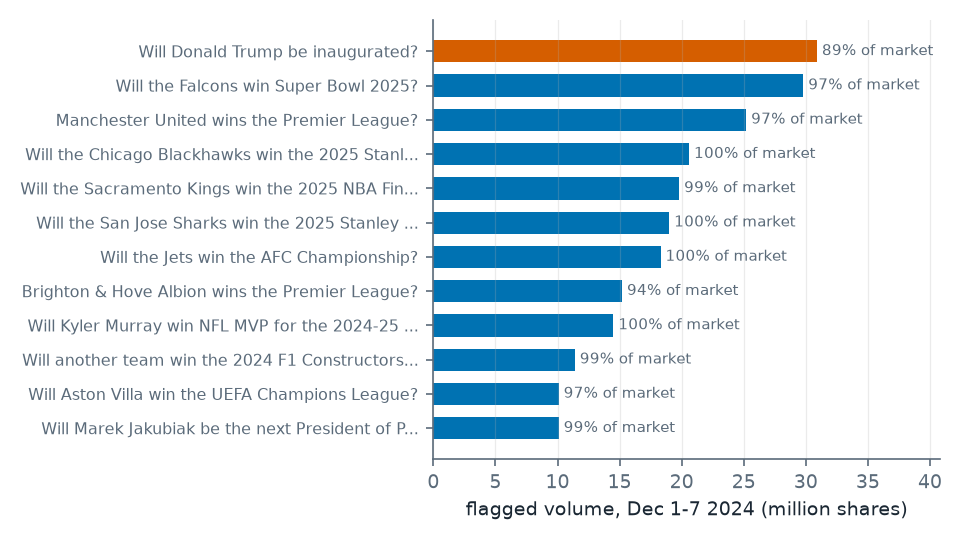
\includegraphics[width=0.92\textwidth]{top_markets}
\caption{ตลาดที่มี volume ถูกติดธงมากที่สุดในสัปดาห์พีคเป็นตลาดกีฬาแบบ ``โอกาสน้อย''
เกือบทั้งหมด และในตลาดเหล่านี้ 94--100\% ของ volume ถูกติดธง
แต่ไม่มีตลาดไหนครองเกิน 7.2\% ของ wash ทั้งหมด --- wash กระจายอยู่ใน 659 จาก 2,307 ตลาด}
\end{figure}

รูปแบบนี้สอดคล้องกับที่เปเปอร์พบว่าตลาดกีฬามี wash ราว 45\% ของ volume
ตลาดโอกาสน้อยราคาต่ำและนิ่ง จึงเทรดวนไปมาได้โดยแทบไม่เสียเงิน

\subsection{ตลาด Trump: จุดที่เราไม่ตรงกับเปเปอร์}
\label{sec:trump}

\begin{warnbox}[title={``Will Donald Trump be inaugurated?'' ถูกติดธง 89\% แต่เปเปอร์ไม่ติดธงเลย}]
Algorithm 2 ของเปเปอร์ไม่พบ $\theta$ ไหนผ่านการทดสอบ spillover ในตลาดนี้ จึงไม่ติดธงเลย
สาเหตุที่น่าจะเป็นมีสองอย่าง
(1) เราใช้ $\theta$ คงที่แทน $\theta$ รายตลาด
(2) ตลาดนี้เปิดยาวมาก lead-in 1 เดือนของเราจึงอาจนับ closure เกินจริง (§\ref{sec:closure})
\textbf{แผน:} คน \rB{} ทำ Algorithm 2 ในเฟส 2 แล้วตรวจตลาดนี้ซ้ำ
ไม่ว่าผลจะออกมาทางไหน นี่เป็นเนื้อหาที่ดีสำหรับ Q\&A และหัวข้อข้อจำกัดในรายงาน
\end{warnbox}

\section{ข้อจำกัดที่ต้องพูดทุกครั้งที่อ้างผลนี้}

\begin{enumerate}
\item \textbf{ไม่มี ground truth} --- ตัวเลขเทียบมาจากเปเปอร์เดียว (SSRN preprint)
      ซึ่งเขียนเองว่าไม่มีป้ายคำตอบ
\item \textbf{position ก่อน lead-in ไม่รู้} --- กระทบตลาดที่เปิดยาวมากที่สุด
\item \textbf{$\theta$ คงที่} --- ยังไม่ใช่ Algorithm 2 ของเปเปอร์
\item \textbf{สองสัปดาห์ยังไม่ใช่ซีรีส์} --- เฟส 2 จะขยายเป็นรายสัปดาห์ตลอด
      พ.ย.--ธ.ค. 2024 และ พ.ค.--มิ.ย. 2025
\end{enumerate}

% =====================================================================
%  PART 4 — THE PLAN
% =====================================================================
\clearpage
\part{แผนงาน: ใครทำอะไร เสร็จเมื่อไร}

\textbf{คำถามของภาคนี้: จากวันนี้ถึง 19 ต.ค. แต่ละคนต้องส่งมอบอะไร ให้ใคร วันไหน?}

\section{ไทม์ไลน์}

\begin{figure}[H]
\centering
\begin{tikzpicture}[x=0.6cm,y=0.62cm]
  % วันที่ d: 30 ก.ย. = 0, 1 ต.ค. = 1, ..., 19 ต.ค. = 19
  % แถบวันหยุดสุดสัปดาห์ (ส.–อา.)
  \foreach \d in {3,10,17}{
    \fill[muted!7] (\d,0.4) rectangle (\d+2,-11.6);
  }
  % แกนวันที่
  \foreach \d/\t in {0/30,2/2,4/4,6/6,8/8,10/10,12/12,14/14,16/16,18/18}{
    \node[lbl] at (\d+0.5,0.9) {\t};
  }
  \node[lbl, anchor=east] at (-0.2,0.9) {ก.ย. / ต.ค.};
  \draw[rule] (0,0.4) -- (20,0.4);

  % แถว: ชื่อ, ช่วง, สี
  \newcommand{\gbar}[5]{% row, start, end(inclusive), colour, label
    \fill[#4!55, rounded corners=1.5pt] (#2+0.08,-#1+0.3) rectangle (#3+0.92,-#1-0.3);
    \node[font=\sansall\scriptsize, anchor=east, text=ink] at (-0.2,-#1) {#5};
  }
  \gbar{0}{0}{1}{muted}{0 ตั้งต้น (ทุกคน)}
  % เฟส 1: แผนเดิม 1–4 ต.ค. (จาง) · เสร็จจริง 30 ก.ย. (เข้ม)
  \fill[evalc!18, rounded corners=1.5pt] (1.08,-0.7) rectangle (4.92,-1.3);
  \fill[evalc!80, rounded corners=1.5pt] (0.08,-0.7) rectangle (0.92,-1.3);
  \node[font=\sansall\scriptsize, anchor=east, text=ink] at (-0.2,-1) {1 premise test (\rA+\rB)};
  \node[lbl, text=evalc!70!black, anchor=west] at (5.1,-1) {เสร็จแล้ว 30 ก.ย.};

  % EDA: รอบแรก 1–4 ต.ค. (เข้ม) · รอบสองบนช่วงเต็ม 8–10 ต.ค. (จาง)
  \gbar{2}{1}{4}{ext}{1--2 EDA (\rC)}
  \fill[ext!25, rounded corners=1.5pt] (8.08,-1.7) rectangle (10.92,-2.3);
  \gbar{3}{5}{7}{accent}{2 ไปป์ไลน์เต็มช่วง (\rA)}
  \gbar{4}{5}{8}{alg}{2 Algorithm 1+2 (\rB)}
  \gbar{5}{5}{9}{ext}{2 chip dumping (\rC)}
  \gbar{6}{10}{10}{muted}{2 รวม notebook demo}
  \gbar{7}{8}{12}{evalc}{3 evaluation (\rB, \rC)}
  \gbar{8}{10}{14}{ext}{4 สไลด์ (\rA+\rC)}
  \gbar{9}{10}{15}{alg}{4 รายงาน (\rB+\rA)}
  \gbar{10}{16}{16}{accent}{4 วิดีโอ (ทุกคน)}
  \gbar{11}{17}{18}{muted}{5 buffer + Q\&A}

  % หมุด: ส่งหัวข้อ และ ส่งงาน
  \foreach \d/\t in {5/ส่งหัวข้อ, 19/ส่งงาน}{
    \draw[bad, line width=1pt] (\d+0.5,0.4) -- (\d+0.5,-11.6);
    \node[tag, text=bad, fill=white, inner sep=1pt] at (\d+0.5,-12.1) {\t};
  }
  \node[lbl, anchor=west] at (0,-12.9) {แถบเทา = เสาร์--อาทิตย์};
\end{tikzpicture}
\caption{ไทม์ไลน์ 30 ก.ย. -- 19 ต.ค. สีของแถบตรงกับสีของเจ้าของงาน
--- premise test เสร็จก่อนกำหนด 4 วัน ทำให้เฟส 2 เริ่มก่อนวันที่ 5 ได้ถ้าทุกคนพร้อม
และ EDA เริ่มได้ทันทีบนข้อมูลสองสัปดาห์ที่มีอยู่}
\end{figure}

\begin{table}[H]
\centering\small
\begin{tabular}{L{4.6cm}L{2.8cm}L{2.2cm}L{4.4cm}}
\toprule
\thd{เฟส} & \thd{วันที่} & \thd{เจ้าของ} & \thd{สถานะ} \\
\midrule
0 ตั้งต้น: โครงโปรเจกต์ บทบาท Drive ถาม TA & 30 ก.ย. -- 1 ต.ค. & ทุกคน & โครงโปรเจกต์เสร็จ รอประชุม \\
1 Premise test & 1 -- 4 ต.ค. & \rA{} + \rB & \textcolor{evalc!70!black}{\textbf{ผ่านแล้ว 30 ก.ย.}} \\
1--2 EDA (รอบแรก · รอบสอง) & 1 -- 4 · 8 -- 10 ต.ค. & \rC & เริ่มได้ทันที \\
\textbf{ส่งหัวข้อ + รายชื่อ} & \textbf{จ. 5 ต.ค.} & ทุกคน & ยังไม่ส่ง \\
2 ไปป์ไลน์เต็มช่วง & 5 -- 10 ต.ค. & \rA, \rB, \rC & ยังไม่เริ่ม \\
3 Evaluation & 8 -- 12 ต.ค. & \rB{} (+\rC) & ยังไม่เริ่ม \\
4 สไลด์ (14) · รายงาน (15) · วิดีโอ (16) & 10 -- 16 ต.ค. & ทุกคน & ยังไม่เริ่ม \\
5 Buffer + เตรียม Q\&A & 17 -- 18 ต.ค. & ทุกคน & --- \\
\textbf{ส่ง Video + PPT + Report} & \textbf{จ. 19 ต.ค.} & ทุกคน & --- \\
\bottomrule
\end{tabular}
\caption{ไทม์ไลน์แบบตาราง (ตรงกับ \code{PROGRESS.md})}
\end{table}

\section{งานของแต่ละคน}

ทุกงานมี\textbf{ของที่ต้องส่งมอบ}ที่ตรวจได้ ไม่ใช่แค่ ``ทำส่วนนี้''
ช่องชื่อเว้นไว้ให้ตกลงกันในที่ประชุม

\subsection{\rA{} --- ไปป์ไลน์ข้อมูล \quad {\normalfont\small\color{muted}ชื่อ: \rule{4cm}{0.4pt}}}

\begin{table}[H]
\centering\small
\begin{tabular}{L{8.2cm}L{4.2cm}L{1.8cm}}
\toprule
\thd{งาน} & \thd{ส่งมอบ} & \thd{เสร็จ} \\
\midrule
ขยายการดึงข้อมูลเป็นทั้ง พ.ย.--ธ.ค. 2024 และ พ.ค.--มิ.ย. 2025 เป็นรายสัปดาห์ &
  parquet เทรดสะอาดรายหน้าต่าง & 7 ต.ค. \\
\addlinespace
ลองขยาย lead-in หรือกรองเฉพาะตลาดที่ทั้งอายุอยู่ในช่วง (\code{startDate}/\code{endDate}) &
  ตัวเลขว่าผลเปลี่ยนเท่าไร & 7 ต.ค. \\
\addlinespace
สุ่มเทียบ position ที่คำนวณเองกับตาราง \code{user\_position} &
  \% ที่ตรงกัน & 7 ต.ค. \\
\addlinespace
เก็บตัวเลขก่อน--หลังทุกขั้น & เนื้อสไลด์ Pre-processing & 7 ต.ค. \\
\addlinespace
สไลด์ Pre-processing + ช่วยรายงาน & 2--3 สไลด์ + 2 หน้า & 14--15 ต.ค. \\
\bottomrule
\end{tabular}
\end{table}

\subsection{\rB{} --- อัลกอริทึมและ evaluation \quad {\normalfont\small\color{muted}ชื่อ: \rule{4cm}{0.4pt}}}

\begin{table}[H]
\centering\small
\begin{tabular}{L{8.2cm}L{4.2cm}L{1.8cm}}
\toprule
\thd{งาน} & \thd{ส่งมอบ} & \thd{เสร็จ} \\
\midrule
Algorithm 1 บนทุกสัปดาห์ของช่วงเต็ม & ซีรีส์ \% ที่ถูกติดธงรายสัปดาห์ & 8 ต.ค. \\
\addlinespace
Algorithm 2 ($\theta$ รายตลาด) + ตรวจตลาด Trump ซ้ำ & ผลเทียบ $\theta$ คงที่ vs รายตลาด & 8 ต.ค. \\
\addlinespace
Evaluation 1: plot ทับ Fig.~7 ของเปเปอร์ & กราฟ + คำอธิบายส่วนต่าง & 10 ต.ค. \\
\addlinespace
Evaluation 2: synthetic injection & precision/recall curve & 12 ต.ค. \\
\addlinespace
คำนวณ precision@k จากผลตรวจมือของ \rC & ตัวเลข precision@k & 12 ต.ค. \\
\addlinespace
รายงาน (เจ้าของหลัก) & PDF 10--15 หน้า & 15 ต.ค. \\
\bottomrule
\end{tabular}
\end{table}

\subsection{\rC{} --- EDA และ chip dumping \quad {\normalfont\small\color{muted}ชื่อ: \rule{4cm}{0.4pt}}}

\begin{table}[H]
\centering\small
\begin{tabular}{L{8.2cm}L{4.2cm}L{1.8cm}}
\toprule
\thd{งาน} & \thd{ส่งมอบ} & \thd{เสร็จ} \\
\midrule
EDA รอบแรกบนข้อมูลสองสัปดาห์ที่มีอยู่ (§\ref{sec:eda}) & 4--6 กราฟ + ข้อสังเกตถึง \rA/\rB & 4 ต.ค. \\
\addlinespace
EDA รอบสองบนช่วงเต็ม + เทียบกระเป๋าที่ถูก/ไม่ถูกติดธง & กราฟชุดสไลด์ Exploration & 10 ต.ค. \\
\addlinespace
กราฟ net value-flow \ensuremath{\to} Louvain & รายการ community ที่น่าสงสัย & 9 ต.ค. \\
\addlinespace
ฟีเจอร์รายกระเป๋า \ensuremath{\to} Isolation Forest + k-means/DBSCAN & ตารางกลุ่ม + คะแนนผิดปกติ & 9 ต.ค. \\
\addlinespace
เขียนเกณฑ์ตรวจมือ (ก่อนดูผล) แล้วตรวจ top-$k$ & ไฟล์เกณฑ์ + ผลตรวจราย wallet & 11 ต.ค. \\
\addlinespace
สไลด์ Complex data, Exploration, Applications (เจ้าของหลักสไลด์) & PPT ครบ 8 ส่วน & 14 ต.ค. \\
\bottomrule
\end{tabular}
\end{table}

\subsection{ใครรอใคร}

\begin{figure}[H]
\centering
\begin{tikzpicture}[x=1cm,y=1cm]
  % แถวบน = เส้นทางวิกฤต · แถวล่าง = งานของ C ที่แตกออกมา
  \node[blk, fill=accent!10, draw=accent!45, text width=2.5cm] (a1) at (0,0)
       {เทรดสะอาดเต็มช่วง\\\scriptsize\rA{} · 7 ต.ค.};
  \node[blk, fill=alg!10, draw=alg!45, text width=2.5cm] (b1) at (3.5,0)
       {ซีรีส์รายสัปดาห์\\\scriptsize\rB{} · 8 ต.ค.};
  \node[blk, fill=evalc!10, draw=evalc!45, text width=2.5cm] (e1) at (7.0,0)
       {evaluation 3 แบบ\\\scriptsize\rB{} · 12 ต.ค.};
  \node[blk, fill=muted!8, draw=muted!40, text width=2.5cm] (d1) at (10.8,-1.1)
       {สไลด์ · รายงาน · วิดีโอ\\\scriptsize ทุกคน · 14--16 ต.ค.};
  \node[blk, fill=ext!10, draw=ext!45, text width=2.5cm] (c1) at (3.5,-2.2)
       {Louvain / IF\\\scriptsize\rC{} · 9 ต.ค.};
  \node[blk, fill=ext!10, draw=ext!45, text width=2.5cm] (c0) at (0,-2.2)
       {EDA รอบแรก\\\scriptsize\rC{} · 4 ต.ค. · ไม่รอใคร};
  \node[blk, fill=ext!10, draw=ext!45, text width=2.5cm] (c2) at (7.0,-2.2)
       {ตรวจมือ top-$k$\\\scriptsize\rC{} · 11 ต.ค.};

  \draw[ar, line width=1.2pt, draw=ink!70] (a1) -- (b1);
  \draw[ar, line width=1.2pt, draw=ink!70] (b1) -- (e1);
  \draw[ar, line width=1.2pt, draw=ink!70] (e1.east) -| (d1.north);
  \draw[ar] (a1.south east) -- (c1.north west);
  \draw[ar, dashed] (c0.north) -- node[lbl, left=1pt] {ข้อสังเกต} (a1.south);
  \draw[ar] (b1) -- (c1);
  \draw[ar] (b1.south east) -- (c2.north west);
  \draw[ar] (c2) -- (e1);
  \draw[ar] (c1.south) -- ++(0,-0.45) -| (d1.south);
  \node[lbl, anchor=south] at (5.25,0.55) {เส้นหนา = เส้นทางวิกฤต};
\end{tikzpicture}
\caption{เส้นทางวิกฤตคือ \rA{} \ensuremath{\to} \rB{} \ensuremath{\to} evaluation \ensuremath{\to} งานส่ง ---
ถ้า \rA{} ช้าหนึ่งวัน ทุกอย่างช้าหนึ่งวัน ระหว่างรอ \rB{} และ \rC{}
ทำงานบนข้อมูลสองสัปดาห์ของ premise test ไปก่อนได้เลย}
\end{figure}

\section{ความเสี่ยงและลำดับการตัด}
\label{sec:risk}

\begin{table}[H]
\centering\small
\begin{tabular}{L{4.6cm}L{2.0cm}L{7.6cm}}
\toprule
\thd{ความเสี่ยง} & \thd{โอกาส} & \thd{รับมืออย่างไร} \\
\midrule
TA ตอบว่ารูปแบบงานต่างจากที่สมมติ & กลาง & ถามให้ได้คำตอบก่อน 5 ต.ค. เหลือเวลาปรับสองสัปดาห์ \\
\addlinespace
ขยายเป็นช่วงเต็มแล้วตัวเลขเปลี่ยนมาก & ต่ำ & premise test ผ่านชัดเจนแล้ว ถ้าเปลี่ยนให้ตรวจ lead-in ก่อน \\
\addlinespace
Algorithm 2 เขียนไม่ทัน / ตีความสเปกไม่ออก & กลาง & ใช้ $\theta$ คงที่ต่อ และรายงานการวิเคราะห์ความไวต่อ $\theta$ แทน \\
\addlinespace
synthetic injection ได้ recall = 0 & ต่ำ & แปลว่าอัลกอริทึมพัง --- หยุดทุกอย่างแล้วไล่บั๊กตามลำดับ
  เทรด \ensuremath{\to} position \ensuremath{\to} closure \ensuremath{\to} คะแนน \\
\addlinespace
คนใดคนหนึ่งติดสอบ/ป่วย & กลาง & มี slack 2 วัน (17--18 ต.ค.) + ตัดงานตามลำดับข้างล่าง \\
\bottomrule
\end{tabular}
\caption{ความเสี่ยงหลัก --- ความเสี่ยงใหญ่ที่สุด (อัลกอริทึมไม่เวิร์ก) ถูกปิดไปแล้วด้วย premise test}
\end{table}

\begin{keybox}[title={ถ้าช้า ตัดตามลำดับนี้ --- และห้ามตัดสองอย่าง}]
\textbf{ตัดได้ตามลำดับ:} (1) ช่วงเสริม ต.ค. 2025 \ensuremath{\to} (2) Isolation Forest
\ensuremath{\to} (3) Algorithm 2 (เหลือ $\theta$ คงที่ + sensitivity)\\[3pt]
\textbf{ห้ามตัด:} Algorithm 1 และ evaluation ทั้งสามแบบ --- สองอย่างนี้คือ 40\% ของคะแนน
และเป็นคำตอบของคำถามแรกที่อาจารย์จะถาม
\end{keybox}

\section{เตรียม Q\&A ไว้ตั้งแต่ตอนนี้}

\begin{table}[H]
\centering\small
\begin{tabular}{L{4.6cm}L{9.6cm}}
\toprule
\thd{คำถามที่คาดว่าจะโดน} & \thd{คำตอบของกลุ่ม} \\
\midrule
ไม่มี ground truth แล้วรู้ได้อย่างไรว่าถูก? &
  evaluation สามแบบ (เทียบเปเปอร์ · injection · precision@k) และความต่างระหว่างสัปดาห์พีคกับสัปดาห์เงียบ \\
\addlinespace
ต่างจากเปเปอร์อย่างไร? &
  ทำซ้ำด้วยข้อมูลคนละแหล่งและโค้ดที่เขียนเอง · เพิ่มมุม chip dumping · เพิ่ม clustering ·
  เจอจุดที่ไม่ตรงกัน (ตลาด Trump) และอธิบายได้ \\
\addlinespace
ทำไม $\theta = 0.9$? &
  เป็นค่าที่เปเปอร์ใช้ และรูป sensitivity แสดงว่าข้อสรุปไม่เปลี่ยนตลอด $\theta \in [0.8, 0.99]$ \\
\addlinespace
ทำไมไม่ใช้ supervised learning? &
  ไม่มีป้ายคำตอบ วิธีที่ใช้ได้จึงต้องเป็น unsupervised / graph-based \\
\addlinespace
ผู้เล่นที่เก็งกำไรระยะสั้นจะโดนติดธงผิดไหม? &
  คะแนนตั้งต้นสูงได้ แต่ชั้นเครือข่ายจะดึงลงถ้าคู่เทรดเป็นคนทั่วไป (รูปที่~\ref{fig:score}) \\
\bottomrule
\end{tabular}
\caption{คำถามที่น่าจะโดนถามและคำตอบที่กลุ่มจะใช้ร่วมกัน --- ทุกคนควรตอบข้อแรกได้}
\end{table}

\section{สิ่งที่ต้องตกลงในที่ประชุมครั้งนี้}

\begin{enumerate}
\item \textbf{ใครเป็น \rA{}, \rB{}, \rC{}} --- เติมชื่อในหัวข้อ ``งานของแต่ละคน''
\item \textbf{ชื่อหัวข้อที่จะส่ง} --- ยืนยันตามหน้าแรก หรือแก้คำ
\item \textbf{ใครถาม TA} (พี่เจม \code{jetana.s@ku.th}) และส่งภายในวันไหน
\item \textbf{สร้างโฟลเดอร์ Drive} \code{GroupXX\_ProjectName/} และแชร์ให้ครบ
\item \textbf{วิธีทำงานร่วมกันบน git} --- แต่ละคนทำ branch ของตัวเอง แล้ว merge เข้า \code{project/polymarket-wash}
\item \textbf{นัดเช็กความคืบหน้า} --- เสนอสั้น ๆ 15 นาที ทุกวันที่ 7, 10, 12, 14 ต.ค.
\item \textbf{AI Usage Log} --- ทุกคนบันทึกลง \code{05\_AI\_Usage\_Log/log.md} ทันทีที่ใช้ AI
\end{enumerate}

\section{นิยามของคำว่า ``เสร็จ'' ก่อนส่ง}

\begin{itemize}
\item[$\square$] ตัวเลขทุกตัวในสไลด์และรายงานมาจากผลรันจริงใน \code{04\_Evaluation/}
\item[$\square$] \% คู่เทรดที่กู้ได้ $\approx$ 100\% และ position ที่สุ่มเทียบตรงกับ \code{user\_position}
\item[$\square$] synthetic injection ได้ recall มากกว่า 0 อย่างชัดเจน
\item[$\square$] notebook demo รันจากเครื่องสะอาดได้จบ
      (\code{uv run jupyter nbconvert --execute})
\item[$\square$] สไลด์ครบ 8 ส่วนของ template · รายงาน 10--15 หน้า · วิดีโอ 8--15 นาที
\item[$\square$] ทุกข้อใน rubric ชี้ไปที่สไลด์หรือหัวข้อรายงานที่ตอบได้ (ใช้ตาราง rubric ในภาคที่ 1 เป็น checklist)
\item[$\square$] AI Usage Log อย่างน้อย 5 prompts
\end{itemize}

% =====================================================================
%  APPENDICES
% =====================================================================
\clearpage
\appendix
\part*{ภาคผนวก}
\addcontentsline{toc}{part}{ภาคผนวก}

\section{อภิธานศัพท์ ไทย--อังกฤษ}

\begin{longtable}{L{4.0cm}L{3.8cm}L{6.6cm}}
\toprule
\thd{ไทย} & \thd{อังกฤษ} & \thd{ความหมายย่อ} \\
\midrule
\endfirsthead
\toprule
\thd{ไทย} & \thd{อังกฤษ} & \thd{ความหมายย่อ} \\
\midrule
\endhead
\bottomrule
\endfoot
การซื้อขายสมรู้ร่วมคิด & wash trading & เทรดกับตัวเองหรือพวกเดียวกันเพื่อสร้าง volume ปลอม \\
การโอนมูลค่าแฝง & chip dumping & ตั้งใจเทรดขาดทุนเพื่อโอนเงินให้อีกกระเป๋า \\
ตลาดทำนายผล & prediction market & ตลาดที่ซื้อขายหุ้นของผลลัพธ์ในอนาคต \\
กระเป๋า & wallet & address บนบล็อกเชน หนึ่งคนมีได้หลายใบ \\
ผู้ตั้งคำสั่ง / ผู้รับคำสั่ง & maker / taker & ฝั่งที่วางคำสั่งไว้ในสมุด / ฝั่งที่มากินคำสั่ง \\
การจับคู่คำสั่ง & fill / match & หนึ่งเหตุการณ์ที่คำสั่งสองฝั่งถูกจับคู่กัน \\
สร้างหุ้นคู่ / รวมหุ้นคู่ & mint / merge & ซื้อ Yes + No พร้อมกัน / ขาย Yes + No พร้อมกัน \\
สถานะการถือ & position & จำนวนหุ้น Yes สุทธิที่กระเป๋าถืออยู่ในตลาดหนึ่ง \\
การปิดสถานะ & closure & position ลดเหลือ $\le$ 0.5\% ของจุดสูงสุด หรือกลับฝั่ง \\
ช่วงข้อมูลเผื่อ & lead-in & ข้อมูลก่อนสัปดาห์เป้าหมายที่ใช้เรียนรู้ position และคะแนน \\
เกณฑ์ตัดสิน & threshold ($\theta$) & คะแนนขั้นต่ำที่ทั้งสองฝั่งต้องมีจึงติดธง \\
การทดสอบสมมติฐานตั้งต้น & premise test & การทดลองเล็กที่ตัดสินว่าจะเลือกหัวข้อนี้หรือไม่ \\
การฝังข้อมูลสังเคราะห์ & synthetic injection & ใส่วง wash ที่รู้คำตอบลงข้อมูลจริงเพื่อวัด recall \\
ความแม่นยำที่ $k$ อันดับแรก & precision@k & สัดส่วนที่ถูกจริงใน $k$ รายการที่ถูกจัดอันดับสูงสุด \\
การหากลุ่มในกราฟ & community detection (Louvain) & แบ่งโหนดเป็นกลุ่มที่เชื่อมกันหนาแน่น \\
ป่าแยกความผิดปกติ & Isolation Forest & หาจุดผิดปกติจากจำนวนครั้งที่ต้องสุ่มแบ่งจนแยกได้ \\
ข้อมูลจริงที่ใช้ตรวจ & ground truth & ป้ายคำตอบที่ถูกต้อง --- งานนี้ไม่มี \\
\end{longtable}

\section{การรันโค้ดจริง}

ทุกคำสั่งรันจากโฟลเดอร์ \code{Project/} (โปรเจกต์ใช้ \code{uv})

\begin{enumerate}
\item ดาวน์โหลดข้อมูลดิบครั้งเดียวลง \code{data/raw/} ตามคำสั่งใน \code{01\_Raw\_Data/README.md}
      (ห้ามดึงเดือนปี 2026)
\item \code{cd 04\_Evaluation/premise\_test \&\& uv run python 01\_extract.py} ---
      fill ดิบ \ensuremath{\to} ตารางเทรดสะอาดใน \code{data/interim/} (คน \rA)
\item \code{uv run python 02\_alg1.py} ---
      closure \ensuremath{\to} คะแนน \ensuremath{\to} \% ที่ถูกติดธง\newline ผลลง \code{results/alg1\_results.json} (คน \rB)
\item \code{cd ../.. \&\& uv run python plan/make\_figures.py} --- สร้างรูปในเอกสารนี้ใหม่
\item \code{cd plan \&\& latexmk -xelatex -outdir=build group\_plan.tex} --- build PDF นี้
\end{enumerate}

\section{เอกสารอ้างอิงหลัก}

\begin{table}[H]
\centering\small
\begin{tabular}{L{5.4cm}L{8.8cm}}
\toprule
\thd{แหล่ง} & \thd{เกี่ยวข้องอย่างไร} \\
\midrule
Sirolly, Ma, Kanoria \& Sethi (2025) \newline \emph{Network-Based Detection of Wash Trading},
SSRN 5714122 &
  สเปกของ Algorithm 1--2 (§5.1, §6) และตัวเลขรายสัปดาห์ (Fig.~7) ที่ใช้เทียบ
  \textbf{ต้องอ้างเป็นงานตั้งต้นที่โครงงานนี้ทำซ้ำและขยาย} \\
\addlinespace
\code{moose-code/polymarket-onchain-v1} \newline Hugging Face, CC-BY-4.0 &
  แหล่งข้อมูลทั้งหมด --- event on-chain ชุดเดียวกับที่เปเปอร์ใช้ แต่คนละช่องทาง \\
\addlinespace
ข่าว CoinDesk / Fortune (พ.ย. 2025) &
  ที่มาของเรื่องเล่า ``หนึ่งในสี่ของ volume อาจเป็นของปลอม'' สำหรับบทนำและวิดีโอ \\
\addlinespace
Blondel et al. (2008) --- Louvain &
  วิธีหา community ในส่วนขยาย \\
\addlinespace
Liu, Ting \& Zhou (2008) --- Isolation Forest &
  วิธีหาความผิดปกติในส่วนขยาย \\
\bottomrule
\end{tabular}
\end{table}

\begin{keybox}[title={เอกสารภายในโครงงานที่ควรอ่านคู่กัน}]
\begin{itemize}
\item \code{PROGRESS.md} --- สถานะล่าสุดและ ``การตัดสินใจที่ห้ามกลับโดยไม่บอก''
\item \code{04\_Evaluation/premise\_test/config.py} --- พารามิเตอร์และหน้าต่างเวลาทั้งหมด
\item \code{01\_Raw\_Data/README.md} --- วิธีดาวน์โหลดข้อมูลและความหมายของแต่ละฟิลด์
\item \code{05\_AI\_Usage\_Log/log.md} --- บันทึกการใช้ AI (ทุกคนเติม)
\end{itemize}
\end{keybox}

\vspace{2em}
\begin{center}
\begin{tikzpicture}
  \draw[rule, line width=0.6pt] (0,0) -- (\textwidth,0);
\end{tikzpicture}
\end{center}
{\sansall\footnotesize\color{muted}
เอกสารนี้สร้างจากโค้ดและผลรันจริงใน \code{Project/04\_Evaluation/premise\_test/}
รูปผลลัพธ์ทั้งสองรูปสร้างใหม่ได้ด้วย \code{plan/make\_figures.py}
ตัวเลขทุกตัวในภาคที่ 3 ตรวจย้อนได้ที่ \code{results/alg1\_results.json}
และ \code{results/extract\_stats.json}\par}

\end{document}
